\documentclass[12pt,a4paper]{article}
\usepackage[utf8]{inputenc}
\usepackage[margin=1in]{geometry}
\usepackage{graphicx}
\usepackage{amsmath}
\usepackage{amssymb}
\usepackage{amsfonts}
\usepackage{booktabs}
\usepackage{longtable}
\usepackage{hyperref}
\usepackage{enumitem}
\usepackage{titlesec}
\usepackage{fancyhdr}
\usepackage{xcolor}
\usepackage{tikz}
\usepackage{pgfplots}
\usepackage{pgfgantt}
\usepackage{quantikz}
\usepackage{circuitikz}

% TikZ Libraries
\usetikzlibrary{shapes.geometric, arrows.meta, positioning, calc, patterns, decorations.pathmorphing, backgrounds, fit, matrix, chains, scopes, decorations.markings}

\pgfplotsset{compat=1.18}

% Custom colors
\definecolor{cdacblue}{RGB}{0, 102, 204}
\definecolor{quantumgreen}{RGB}{0, 153, 76}
\definecolor{fpgaorange}{RGB}{255, 153, 0}
\definecolor{nodered}{RGB}{204, 0, 0}
\definecolor{lightblue}{RGB}{230, 242, 255}
\definecolor{lightgreen}{RGB}{230, 255, 230}
\definecolor{lightorange}{RGB}{255, 243, 230}
\definecolor{lightred}{RGB}{255, 230, 230}

% TikZ Styles
\tikzstyle{block} = [rectangle, draw=cdacblue, fill=lightblue, text width=3cm, text centered, rounded corners, minimum height=1cm, line width=1pt]
\tikzstyle{wideblock} = [rectangle, draw=cdacblue, fill=lightblue, text width=4.5cm, text centered, rounded corners, minimum height=1cm, line width=1pt]
\tikzstyle{smallblock} = [rectangle, draw=cdacblue, fill=lightblue, text width=2.5cm, text centered, rounded corners, minimum height=0.8cm, font=\small, line width=1pt]
\tikzstyle{process} = [rectangle, draw=quantumgreen, fill=lightgreen, text width=3cm, text centered, minimum height=1cm, line width=1pt]
\tikzstyle{decision} = [diamond, draw=fpgaorange, fill=lightorange, text width=2cm, text centered, aspect=2, line width=1pt]
\tikzstyle{io} = [trapezium, trapezium left angle=70, trapezium right angle=110, draw=nodered, fill=lightred, text width=2.5cm, text centered, minimum height=0.8cm, line width=1pt]
\tikzstyle{arrow} = [-{Stealth[length=3mm]}, thick]
\tikzstyle{dashedarrow} = [-{Stealth[length=3mm]}, thick, dashed]

\pagestyle{fancy}
\fancyhf{}
\rhead{FPGA-Based Quantum Pulse Simulator}
\lhead{Project Proposal}
\cfoot{\thepage}

\title{\textbf{FPGA-Based Quantum Pulse-Level Simulator:\\Bridging Theoretical Quantum Computing with Physical Hardware Realization}}
\author{Centre for Development of Advanced Computing (C-DAC), Noida}
\date{}

\begin{document}
\maketitle

\section*{Executive Summary}

This proposal presents a three-year research and development initiative to design, implement, and validate an FPGA-based quantum pulse-level simulator capable of modeling quantum operations at the physical control layer. Building upon C-DAC Noida's successful gate-level quantum simulator (30 qubits), this project addresses the critical gap between abstract quantum circuits and physical quantum hardware implementation.

While gate-level simulators operate on idealized quantum gates, real quantum processors function through precisely timed electromagnetic pulses. This pulse simulator will enable:

\begin{itemize}[noitemsep]
    \item Direct emulation of control electronics and pulse sequences used in actual quantum hardware
    \item Realistic modeling of pulse-level errors, crosstalk, and decoherence mechanisms
    \item Optimization of control pulses before deployment on expensive quantum hardware
    \item Hardware-in-the-loop testing for quantum control systems
    \item Indigenous capability in quantum control software stack development
\end{itemize}

The project targets 12-qubit pulse-level simulation with sub-nanosecond timing resolution, incorporating Hamiltonian-based evolution, arbitrary waveform generation, and comprehensive noise characterization.

%% ============ SYSTEM OVERVIEW DIAGRAM ============
\begin{figure}[htbp]
\centering
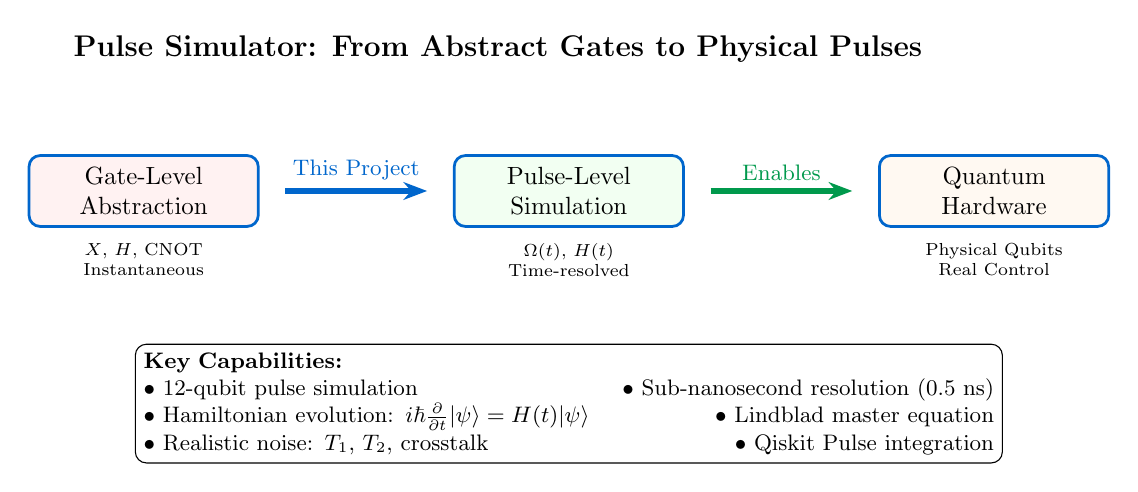
\begin{tikzpicture}[node distance=1.5cm, scale=0.9, transform shape]
    % Title
    \node[font=\large\bfseries] at (0, 4.5) {Pulse Simulator: From Abstract Gates to Physical Pulses};
    
    % Gate Level (Abstract)
    \node[block, fill=lightred!50] (gate) at (-5, 2.5) {Gate-Level\\Abstraction};
    \node[below=0.1cm of gate, font=\scriptsize, text width=3cm, align=center] {$X$, $H$, CNOT\\Instantaneous};
    
    % Arrow
    \draw[arrow, line width=2pt, cdacblue] (-3, 2.5) -- (-1, 2.5) node[midway, above, font=\small] {This Project};
    
    % Pulse Level
    \node[block, fill=lightgreen!50] (pulse) at (1, 2.5) {Pulse-Level\\Simulation};
    \node[below=0.1cm of pulse, font=\scriptsize, text width=3cm, align=center] {$\Omega(t)$, $H(t)$\\Time-resolved};
    
    % Arrow to Hardware
    \draw[arrow, line width=2pt, quantumgreen] (3, 2.5) -- (5, 2.5) node[midway, above, font=\small] {Enables};
    
    % Hardware
    \node[block, fill=lightorange!50] (hw) at (7, 2.5) {Quantum\\Hardware};
    \node[below=0.1cm of hw, font=\scriptsize, text width=3cm, align=center] {Physical Qubits\\Real Control};
    
    % Key Features Box
    \node[draw, rounded corners, fill=white, text width=12cm, align=left, font=\small] at (1, -0.5) {
        \textbf{Key Capabilities:}\\
        $\bullet$ 12-qubit pulse simulation \hfill $\bullet$ Sub-nanosecond resolution (0.5 ns)\\
        $\bullet$ Hamiltonian evolution: $i\hbar\frac{\partial}{\partial t}|\psi\rangle = H(t)|\psi\rangle$ \hfill $\bullet$ Lindblad master equation\\
        $\bullet$ Realistic noise: $T_1$, $T_2$, crosstalk \hfill $\bullet$ Qiskit Pulse integration
    };
\end{tikzpicture}
\caption{Project Overview: Bridging gate-level abstraction to physical hardware through pulse-level simulation}
\label{fig:overview}
\end{figure}

\textbf{Defense of FPGA Approach Despite Hardware Advancement:} Physical quantum hardware deployment is accelerating globally, yet pulse-level simulation remains critical for three fundamental reasons:

\begin{enumerate}[noitemsep]
    \item \textbf{Hardware Calibration and Characterization:} Even with available quantum processors, continuous pulse optimization and calibration requires thousands of iterations. Cloud-based quantum hardware access is expensive, queue-limited, and unsuitable for iterative pulse tuning. FPGA pulse simulators enable local, rapid iteration without hardware access costs or scheduling constraints.
    
    \item \textbf{Realistic Error Modeling:} Gate-level simulators abstract away physical error sources. Pulse simulators capture timing errors, control noise, pulse distortions, crosstalk between qubits, and non-Markovian effects that dominate actual hardware behavior.
    
    \item \textbf{Co-Design and Algorithm Development:} Future quantum advantage requires co-design—algorithms developed with awareness of hardware constraints. Pulse-level simulation enables testing quantum algorithms against realistic pulse sequences.
    
    \item \textbf{Sovereign Technology Stack:} India's quantum computing sovereignty demands indigenous capabilities at every layer—from silicon to software.
    
    \item \textbf{Pedagogical and Workforce Development:} Training quantum engineers requires tools that expose pulse-level physics without requiring access to rare, expensive quantum hardware.
\end{enumerate}

\newpage
\section{Background and Motivation}

\subsection{Current State of Quantum Computing Infrastructure}

C-DAC Noida's gate-level quantum simulator demonstrated India's capability to develop indigenous quantum computing infrastructure. The system achieved:

\begin{itemize}[noitemsep]
    \item 30-qubit state vector simulation using Xilinx Alveo U55C FPGA with HBM architecture
    \item 100\% success rate across all tested configurations
    \item Seamless integration with Qniverse Platform, Qiskit 1.0.2, and Qiskit-Aer 0.14.1
    \item Complete ground-up architecture without reliance on pre-existing frameworks
    \item Validation across 40+ quantum algorithms including VQE, QAOA, Grover, Shor
\end{itemize}

However, gate-level simulation operates at an abstraction layer divorced from physical quantum hardware implementation.

\subsection{The Critical Gap: Gate-Level vs. Pulse-Level}

%% ============ GATE VS PULSE COMPARISON DIAGRAM ============
\begin{figure}[htbp]
\centering
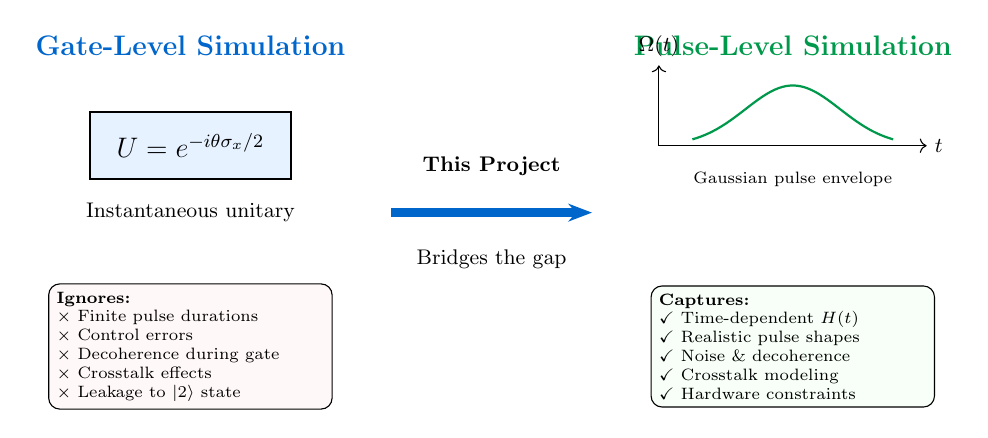
\begin{tikzpicture}[scale=0.85, transform shape]
    % Gate Level Side
    \node[font=\large\bfseries, cdacblue] at (-4.5, 5) {Gate-Level Simulation};
    
    % Gate representation
    \draw[thick, fill=lightblue] (-6, 3) rectangle (-3, 4);
    \node at (-4.5, 3.5) {\large $U = e^{-i\theta\sigma_x/2}$};
    \node[font=\small] at (-4.5, 2.5) {Instantaneous unitary};
    
    % What it ignores
    \node[draw, rounded corners, fill=lightred!30, text width=4cm, align=left, font=\scriptsize] at (-4.5, 0.5) {
        \textbf{Ignores:}\\
        $\times$ Finite pulse durations\\
        $\times$ Control errors\\
        $\times$ Decoherence during gate\\
        $\times$ Crosstalk effects\\
        $\times$ Leakage to $|2\rangle$ state
    };
    
    % Arrow
    \draw[arrow, line width=3pt, cdacblue] (-1.5, 2.5) -- (1.5, 2.5);
    \node[font=\small\bfseries] at (0, 3.2) {This Project};
    \node[font=\small] at (0, 1.8) {Bridges the gap};
    
    % Pulse Level Side
    \node[font=\large\bfseries, quantumgreen] at (4.5, 5) {Pulse-Level Simulation};
    
    % Pulse waveform
    \begin{scope}[shift={(4.5, 3.5)}]
        \draw[->] (-2, 0) -- (2, 0) node[right, font=\small] {$t$};
        \draw[->] (-2, 0) -- (-2, 1.2) node[above, font=\small] {$\Omega(t)$};
        \draw[thick, quantumgreen, domain=-1.5:1.5, samples=50] plot (\x, {0.9*exp(-\x*\x)});
        \node[font=\scriptsize] at (0, -0.5) {Gaussian pulse envelope};
    \end{scope}
    
    % What it captures
    \node[draw, rounded corners, fill=lightgreen!30, text width=4cm, align=left, font=\scriptsize] at (4.5, 0.5) {
        \textbf{Captures:}\\
        $\checkmark$ Time-dependent $H(t)$\\
        $\checkmark$ Realistic pulse shapes\\
        $\checkmark$ Noise \& decoherence\\
        $\checkmark$ Crosstalk modeling\\
        $\checkmark$ Hardware constraints
    };
\end{tikzpicture}
\caption{Comparison between gate-level and pulse-level simulation approaches}
\label{fig:gate-vs-pulse}
\end{figure}

\textbf{Gate-Level Simulation:} Represents quantum operations as unitary matrices applied instantaneously to quantum states. This abstraction is mathematically convenient but physically unrealistic.

\textbf{Pulse-Level Simulation:} Models quantum evolution under time-dependent Hamiltonians driven by control pulses. This approach:
\begin{itemize}[noitemsep]
    \item Solves the Schrödinger equation with realistic pulse waveforms
    \item Captures pulse-induced errors and hardware-specific constraints
    \item Enables optimization of pulse shapes, amplitudes, and phases
    \item Provides direct connection to control electronics and AWG specifications
\end{itemize}

The fidelity gap between idealized gates and actual pulse implementations typically ranges from 0.1\% to 5\% error per gate, which compounds catastrophically in multi-gate circuits.

\subsection{Why Quantum Hardware Availability Strengthens the Case for Pulse Simulation}

%% ============ COST BENEFIT ANALYSIS DIAGRAM ============
\begin{figure}[htbp]
\centering
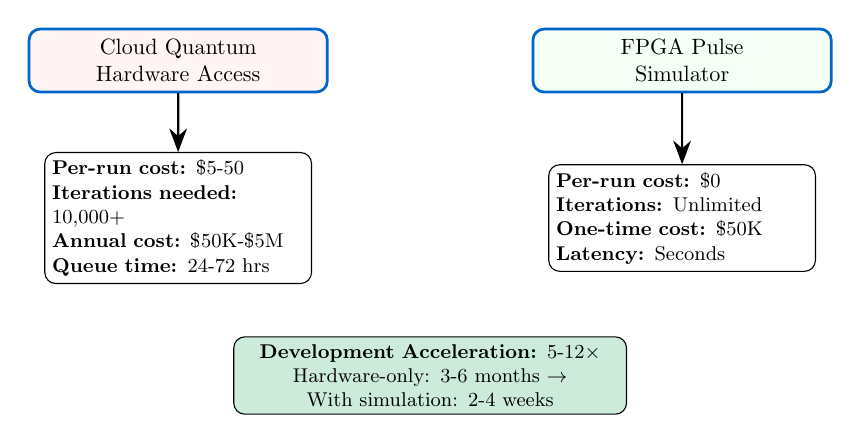
\begin{tikzpicture}[scale=0.8, transform shape]
    % Hardware calibration economics
    \node[wideblock, fill=lightred!40] (cloud) at (-4, 3) {Cloud Quantum\\Hardware Access};
    \node[wideblock, fill=lightgreen!40] (fpga) at (4, 3) {FPGA Pulse\\Simulator};
    
    % Cost comparison
    \node[draw, rounded corners, text width=4cm, font=\small, align=left] (cloudcost) at (-4, 0.5) {
        \textbf{Per-run cost:} \$5-50\\
        \textbf{Iterations needed:} 10,000+\\
        \textbf{Annual cost:} \$50K-\$5M\\
        \textbf{Queue time:} 24-72 hrs
    };
    
    \node[draw, rounded corners, text width=4cm, font=\small, align=left] (fpgacost) at (4, 0.5) {
        \textbf{Per-run cost:} \$0\\
        \textbf{Iterations:} Unlimited\\
        \textbf{One-time cost:} \$50K\\
        \textbf{Latency:} Seconds
    };
    
    \draw[arrow] (cloud) -- (cloudcost);
    \draw[arrow] (fpga) -- (fpgacost);
    
    % Speedup factor
    \node[draw, rounded corners, fill=quantumgreen!20, text width=6cm, align=center, font=\small] at (0, -2) {
        \textbf{Development Acceleration:} 5-12$\times$\\
        Hardware-only: 3-6 months $\rightarrow$ With simulation: 2-4 weeks
    };
\end{tikzpicture}
\caption{Economic and time benefits of FPGA pulse simulation vs. cloud hardware access}
\label{fig:cost-benefit}
\end{figure}

\newpage
\section{Technical Objectives}

This three-year project will deliver a production-grade FPGA-based quantum pulse-level simulator with the following technical specifications:

\subsection{Primary Objectives}

\textbf{Objective 1: Pulse-Level Quantum Evolution Engine}

Design and implement FPGA hardware kernels for solving the time-dependent Schrödinger equation:
\begin{equation}
i\hbar \frac{\partial}{\partial t}|\psi(t)\rangle = H(t)|\psi(t)\rangle
\label{eq:schrodinger}
\end{equation}

where $H(t) = H_0 + \sum_k \Omega_k(t) H_k$ represents the system Hamiltonian with control pulses $\Omega_k(t)$.

\textbf{Target Specifications:}
\begin{itemize}[noitemsep]
    \item System size: 12 qubits (4096-dimensional Hilbert space)
    \item Time resolution: $\leq 0.5$ ns (matching typical AWG sampling rates)
    \item Simulation duration: Up to 1 ms continuous evolution
    \item Integration method: 4th-order Magnus expansion with adaptive time-stepping
    \item Pulse bandwidth: DC to 10 GHz (covering superconducting qubit control range)
\end{itemize}

\textbf{Objective 2: Comprehensive Noise and Decoherence Modeling}

Implement realistic noise channels at the pulse level using the Lindblad master equation:
\begin{equation}
\frac{d\rho}{dt} = -\frac{i}{\hbar}[H(t), \rho] + \sum_k \gamma_k \mathcal{D}[L_k]\rho
\label{eq:lindblad}
\end{equation}

where the Lindblad dissipator is defined as:
\begin{equation}
\mathcal{D}[L]\rho = L\rho L^\dagger - \frac{1}{2}\left(L^\dagger L\rho + \rho L^\dagger L\right)
\label{eq:dissipator}
\end{equation}

Noise models include:
\begin{itemize}[noitemsep]
    \item Amplitude noise: $\Omega(t) \rightarrow \Omega(t)(1 + \epsilon_A(t))$ with $\epsilon_A \sim \mathcal{N}(0, \sigma_A^2)$
    \item Phase noise: $\phi(t) \rightarrow \phi(t) + \epsilon_\phi(t)$ with $\epsilon_\phi \sim \mathcal{N}(0, \sigma_\phi^2)$
    \item Timing jitter: $t \rightarrow t + \delta t$ with $\delta t \sim \mathcal{N}(0, \sigma_t^2)$
    \item $T_1$ (amplitude damping) and $T_2$ (dephasing) processes
    \item Crosstalk matrices for simultaneous multi-qubit operations
\end{itemize}

\textbf{Objective 3: Hardware Platform Architecture}
\begin{itemize}[noitemsep]
    \item Platform: Xilinx Alveo U55C or successor (VU9P Ultrascale+ FPGA with HBM2)
    \item Memory: 16 GB HBM2 with 32 banks for density matrix storage
    \item Compute: Custom HLS kernels for Hamiltonian evaluation, exponential integration
    \item I/O: PCIe Gen4 x16 for host communication (minimum 32 GB/s bidirectional)
    \item Precision: Single-precision (FP32) and double-precision (FP64) configurable
\end{itemize}

\newpage
\section{Technical Approach and Methodology}

\subsection{System Architecture Overview}

%% ============ MAIN SYSTEM ARCHITECTURE DIAGRAM ============
\begin{figure}[htbp]
\centering
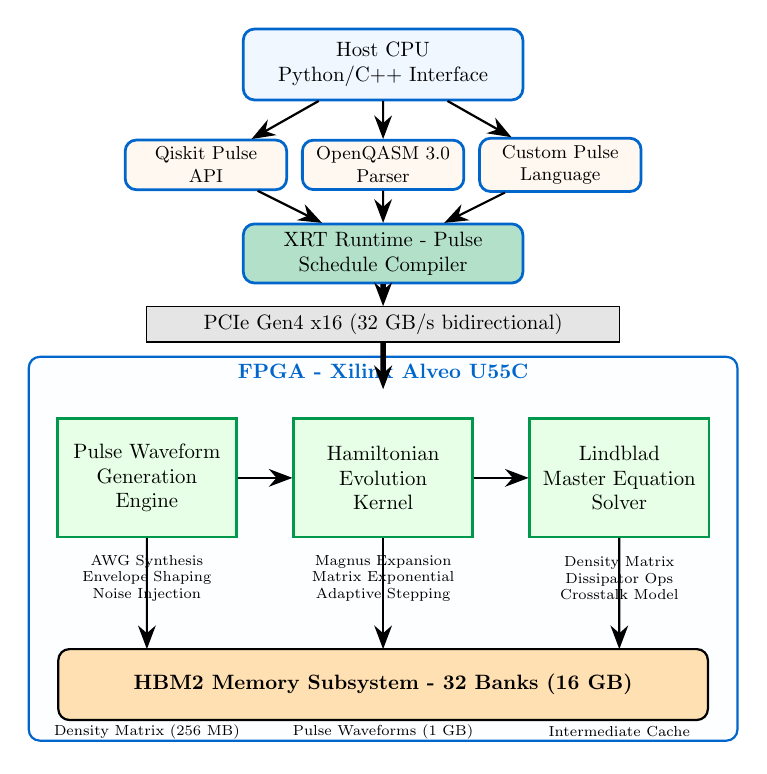
\begin{tikzpicture}[node distance=0.8cm, scale=0.75, transform shape]
    % Host Layer
    \node[wideblock, fill=lightblue!60, minimum height=1.2cm] (host) at (0, 8) {Host CPU\\Python/C++ Interface};
    
    % API Layer
    \node[smallblock, fill=lightorange!60] (qiskit) at (-3, 6.3) {Qiskit Pulse\\API};
    \node[smallblock, fill=lightorange!60] (openqasm) at (0, 6.3) {OpenQASM 3.0\\Parser};
    \node[smallblock, fill=lightorange!60] (custom) at (3, 6.3) {Custom Pulse\\Language};
    
    \draw[arrow] (host) -- (qiskit);
    \draw[arrow] (host) -- (openqasm);
    \draw[arrow] (host) -- (custom);
    
    % XRT Runtime
    \node[wideblock, fill=quantumgreen!30, minimum height=1cm] (xrt) at (0, 4.8) {XRT Runtime - Pulse Schedule Compiler};
    
    \draw[arrow] (qiskit) -- (xrt);
    \draw[arrow] (openqasm) -- (xrt);
    \draw[arrow] (custom) -- (xrt);
    
    % PCIe Interface
    \node[draw, fill=gray!20, minimum width=8cm, minimum height=0.6cm] (pcie) at (0, 3.6) {PCIe Gen4 x16 (32 GB/s bidirectional)};
    
    \draw[arrow, line width=2pt] (xrt) -- (pcie);
    
    % FPGA Main Box
    \node[draw, thick, cdacblue, fill=lightblue!10, minimum width=12cm, minimum height=6.5cm, rounded corners] (fpga) at (0, -0.2) {};
    \node[font=\bfseries, cdacblue] at (0, 2.8) {FPGA - Xilinx Alveo U55C};
    
    \draw[arrow, line width=2pt] (pcie) -- (0, 2.5);
    
    % FPGA Internal Components
    % Waveform Engine
    \node[process, text width=2.8cm, minimum height=2cm] (waveform) at (-4, 1) {Pulse Waveform\\Generation\\Engine};
    \node[font=\scriptsize, text width=2.5cm, align=center] at (-4, -0.7) {AWG Synthesis\\Envelope Shaping\\Noise Injection};
    
    % Hamiltonian Engine
    \node[process, text width=2.8cm, minimum height=2cm] (hamilton) at (0, 1) {Hamiltonian\\Evolution\\Kernel};
    \node[font=\scriptsize, text width=2.5cm, align=center] at (0, -0.7) {Magnus Expansion\\Matrix Exponential\\Adaptive Stepping};
    
    % Lindblad Solver
    \node[process, text width=2.8cm, minimum height=2cm] (lindblad) at (4, 1) {Lindblad\\Master Equation\\Solver};
    \node[font=\scriptsize, text width=2.5cm, align=center] at (4, -0.7) {Density Matrix\\Dissipator Ops\\Crosstalk Model};
    
    % Arrows between engines
    \draw[arrow] (waveform) -- (hamilton);
    \draw[arrow] (hamilton) -- (lindblad);
    
    % HBM Memory
    \node[draw, thick, fill=fpgaorange!30, minimum width=11cm, minimum height=1.2cm, rounded corners] (hbm) at (0, -2.5) {};
    \node[font=\bfseries] at (0, -2.5) {HBM2 Memory Subsystem - 32 Banks (16 GB)};
    
    % HBM banks detail
    \node[font=\scriptsize] at (-4, -3.3) {Density Matrix (256 MB)};
    \node[font=\scriptsize] at (0, -3.3) {Pulse Waveforms (1 GB)};
    \node[font=\scriptsize] at (4, -3.3) {Intermediate Cache};
    
    \draw[arrow] (waveform) -- (-4, -1.9);
    \draw[arrow] (hamilton) -- (0, -1.9);
    \draw[arrow] (lindblad) -- (4, -1.9);
\end{tikzpicture}
\caption{Complete system architecture of the FPGA-based quantum pulse simulator}
\label{fig:system-arch}
\end{figure}

\subsection{Phase 1 Implementation: Core Pulse Evolution Engine (Year 1)}

\subsubsection{Hamiltonian Representation and Storage}

For an $n$-qubit system, the Hamiltonian is decomposed as:
\begin{equation}
H(t) = \underbrace{\sum_{i=1}^n \frac{\omega_i}{2} Z_i + \sum_{i<j} J_{ij} Z_i Z_j}_{H_0 \text{ (static)}} + \underbrace{\sum_k \Omega_k(t) O_k}_{H_{\text{control}}(t)}
\label{eq:hamiltonian}
\end{equation}

where $\omega_i$ are qubit frequencies (typically 4-8 GHz for superconducting qubits), $J_{ij}$ are coupling strengths (10-100 MHz), and $O_k$ are control operators.

%% ============ HAMILTONIAN ENGINE BLOCK DIAGRAM ============
\begin{figure}[htbp]
\centering
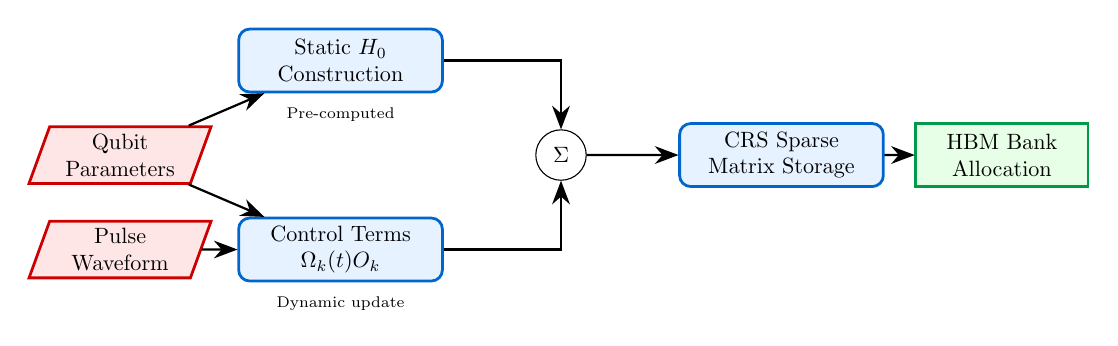
\begin{tikzpicture}[node distance=1cm, scale=0.8, transform shape]
    % Input
    \node[io, text width=2cm] (input) at (-5, 2) {Qubit\\Parameters};
    
    % Static Hamiltonian
    \node[block, text width=3cm] (h0) at (-1.5, 3.5) {Static $H_0$\\Construction};
    
    % Control Terms
    \node[block, text width=3cm] (hc) at (-1.5, 0.5) {Control Terms\\$\Omega_k(t) O_k$};
    
    % Pulse input
    \node[io, text width=2cm] (pulse) at (-5, 0.5) {Pulse\\Waveform};
    
    % Summation
    \node[draw, circle, minimum size=0.8cm] (sum) at (2, 2) {$\Sigma$};
    
    % Sparse Storage
    \node[block, text width=3cm] (sparse) at (5.5, 2) {CRS Sparse\\Matrix Storage};
    
    % HBM
    \node[process, text width=2.5cm] (hbm) at (9, 2) {HBM Bank\\Allocation};
    
    % Arrows
    \draw[arrow] (input) -- (h0);
    \draw[arrow] (input) -- (hc);
    \draw[arrow] (pulse) -- (hc);
    \draw[arrow] (h0) -| (sum);
    \draw[arrow] (hc) -| (sum);
    \draw[arrow] (sum) -- (sparse);
    \draw[arrow] (sparse) -- (hbm);
    
    % Labels
    \node[font=\scriptsize, below=0.1cm of h0] {Pre-computed};
    \node[font=\scriptsize, below=0.1cm of hc] {Dynamic update};
\end{tikzpicture}
\caption{Hamiltonian construction engine block diagram}
\label{fig:hamiltonian-engine}
\end{figure}

\textbf{FPGA Implementation Strategy:}
\begin{itemize}[noitemsep]
    \item Store Hamiltonian terms as sparse matrices in HBM using Compressed Row Storage (CRS)
    \item Pre-compute static Hamiltonian component $H_0$ at initialization
    \item Construct $H(t)$ dynamically by adding control terms weighted by $\Omega_k(t)$
    \item Implement Hamiltonian-vector multiplication using pipelined matrix operations
\end{itemize}

\subsubsection{Time Evolution via Magnus Expansion}

The time evolution operator $U(t, t_0)$ is computed using the Magnus expansion:
\begin{equation}
U(t, t_0) = \exp\left(\Omega(t, t_0)\right)
\label{eq:magnus-main}
\end{equation}

where $\Omega(t, t_0) = \Omega^{[1]} + \Omega^{[2]} + \Omega^{[3]} + \Omega^{[4]} + \ldots$ with:

\textbf{First-order term:}
\begin{equation}
\Omega^{[1]} = -\frac{i}{\hbar} \int_{t_0}^{t} H(\tau) \, d\tau
\label{eq:magnus1}
\end{equation}

\textbf{Second-order term:}
\begin{equation}
\Omega^{[2]} = -\frac{1}{2\hbar^2} \int_{t_0}^{t} d\tau_1 \int_{t_0}^{\tau_1} d\tau_2 \, [H(\tau_1), H(\tau_2)]
\label{eq:magnus2}
\end{equation}

\textbf{Third-order term:}
\begin{equation}
\Omega^{[3]} = \frac{i}{6\hbar^3} \int_{t_0}^{t} d\tau_1 \int_{t_0}^{\tau_1} d\tau_2 \int_{t_0}^{\tau_2} d\tau_3 \left([H(\tau_1), [H(\tau_2), H(\tau_3)]] + [H(\tau_3), [H(\tau_2), H(\tau_1)]]\right)
\label{eq:magnus3}
\end{equation}

\textbf{Fourth-order term:}
\begin{equation}
\Omega^{[4]} = \frac{1}{12\hbar^4} \int_{t_0}^{t} d\tau_1 \cdots \int_{t_0}^{\tau_3} d\tau_4 \left([[[H_1, H_2], H_3], H_4] + [H_1, [[H_2, H_3], H_4]] + \ldots\right)
\label{eq:magnus4}
\end{equation}

where we use $H_i \equiv H(\tau_i)$ for brevity.

%% ============ MAGNUS EXPANSION FLOW DIAGRAM ============
\begin{figure}[htbp]
\centering
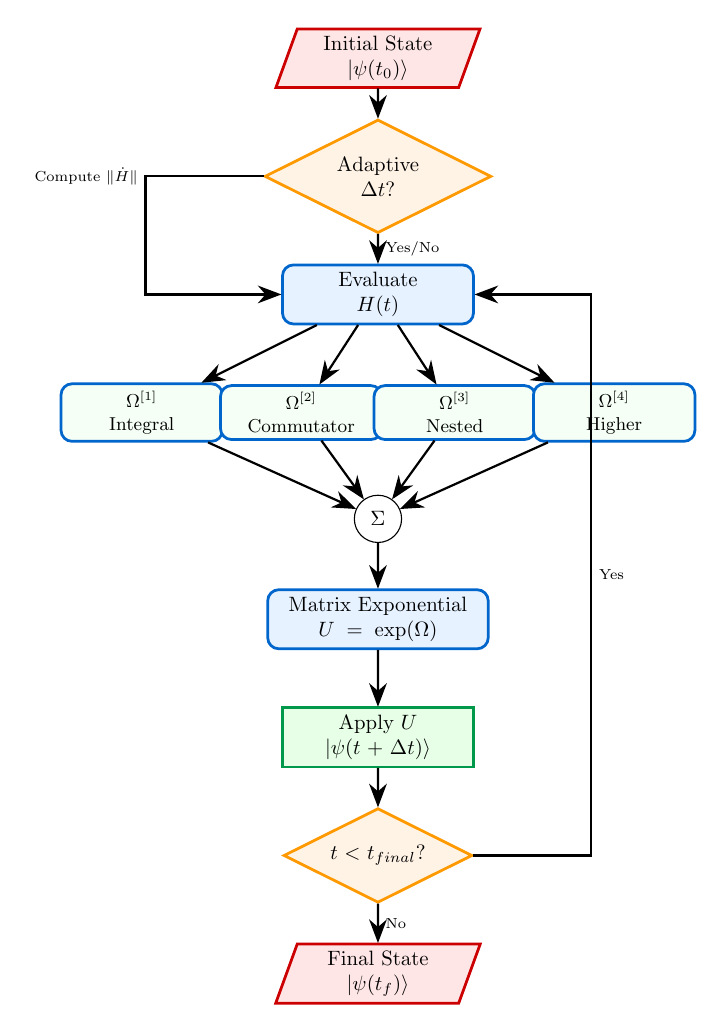
\begin{tikzpicture}[node distance=1.2cm, scale=0.75, transform shape]
    % Start
    \node[io, text width=2.5cm] (start) at (0, 6) {Initial State\\$|\psi(t_0)\rangle$};
    
    % Time step selection
    \node[decision, text width=1.8cm] (adapt) at (0, 4) {Adaptive\\$\Delta t$?};
    
    % Compute H(t)
    \node[block] (ht) at (0, 2) {Evaluate\\$H(t)$};
    
    % Magnus terms - horizontal layout
    \node[smallblock, fill=lightgreen!40] (m1) at (-4, 0) {$\Omega^{[1]}$\\Integral};
    \node[smallblock, fill=lightgreen!40] (m2) at (-1.3, 0) {$\Omega^{[2]}$\\Commutator};
    \node[smallblock, fill=lightgreen!40] (m3) at (1.3, 0) {$\Omega^{[3]}$\\Nested};
    \node[smallblock, fill=lightgreen!40] (m4) at (4, 0) {$\Omega^{[4]}$\\Higher};
    
    % Sum
    \node[draw, circle, minimum size=0.8cm] (sum) at (0, -1.8) {$\Sigma$};
    
    % Matrix exponential
    \node[block, text width=3.5cm] (exp) at (0, -3.5) {Matrix Exponential\\$U = \exp(\Omega)$};
    
    % Apply
    \node[process, text width=3cm] (apply) at (0, -5.5) {Apply $U$\\$|\psi(t+\Delta t)\rangle$};
    
    % Convergence check
    \node[decision, text width=1.8cm] (conv) at (0, -7.5) {$t < t_{final}$?};
    
    % Output
    \node[io, text width=2.5cm] (output) at (0, -9.5) {Final State\\$|\psi(t_f)\rangle$};
    
    % Arrows
    \draw[arrow] (start) -- (adapt);
    \draw[arrow] (adapt) -- (ht) node[midway, right, font=\scriptsize] {Yes/No};
    \draw[arrow] (ht) -- (m1);
    \draw[arrow] (ht) -- (m2);
    \draw[arrow] (ht) -- (m3);
    \draw[arrow] (ht) -- (m4);
    \draw[arrow] (m1) -- (sum);
    \draw[arrow] (m2) -- (sum);
    \draw[arrow] (m3) -- (sum);
    \draw[arrow] (m4) -- (sum);
    \draw[arrow] (sum) -- (exp);
    \draw[arrow] (exp) -- (apply);
    \draw[arrow] (apply) -- (conv);
    \draw[arrow] (conv) -- (output) node[midway, right, font=\scriptsize] {No};
    \draw[arrow] (conv.east) -- ++(2,0) |- (ht.east) node[pos=0.25, right, font=\scriptsize] {Yes};
    
    % Adaptive branch
    \draw[arrow] (adapt.west) -- ++(-2,0) node[left, font=\scriptsize] {Compute $\|\dot{H}\|$} |- (ht.west);
\end{tikzpicture}
\caption{Magnus expansion time evolution algorithm flow diagram}
\label{fig:magnus-flow}
\end{figure}

\textbf{Convergence Analysis:} The Magnus expansion converges when:
\begin{equation}
\int_{t_0}^{t} \|H(\tau)\|_2 \, d\tau < \pi\hbar
\label{eq:magnus-convergence}
\end{equation}

For typical superconducting qubit control with $\|H\| \sim 100$ MHz, this requires $\Delta t \lesssim 5$ ns per Magnus step, well within our 0.5 ns resolution target.

\subsubsection{Matrix Exponential Hardware Acceleration}

Computing $\exp(-iH\Delta t/\hbar)$ is the computational bottleneck. We implement two approaches:

\textbf{Approach A: Eigendecomposition (Exact for Small Systems)}
\begin{equation}
H = V\Lambda V^\dagger \quad \Rightarrow \quad e^{-iHt/\hbar} = V e^{-i\Lambda t/\hbar} V^\dagger
\label{eq:eigendecomp}
\end{equation}

Feasible for $\leq 8$ qubits (256 $\times$ 256 matrices) using Jacobi eigenvalue algorithm.

\textbf{Approach B: Padé Approximation with Scaling and Squaring}

For larger systems, we use the $(p,q)$-Padé approximant:
\begin{equation}
e^{A} \approx R_{p,q}(A) = \left[D_{p,q}(A)\right]^{-1} N_{p,q}(A)
\label{eq:pade}
\end{equation}

where:
\begin{align}
N_{p,q}(A) &= \sum_{j=0}^{p} \frac{(p+q-j)! \, p!}{(p+q)! \, j! \, (p-j)!} A^j \\
D_{p,q}(A) &= \sum_{j=0}^{q} \frac{(p+q-j)! \, q!}{(p+q)! \, j! \, (q-j)!} (-A)^j
\end{align}

\textbf{Scaling and Squaring Algorithm:}
\begin{enumerate}[noitemsep]
    \item Choose $s$ such that $\|A/2^s\| < 1$ (scaling)
    \item Compute $R_{13,13}(A/2^s)$ using (13,13)-Padé approximant
    \item Square $s$ times: $e^A = \left[e^{A/2^s}\right]^{2^s}$ (squaring)
\end{enumerate}

The (13,13)-Padé approximant achieves machine precision for IEEE 754 double-precision.

%% ============ MATRIX EXPONENTIAL BLOCK DIAGRAM ============
\begin{figure}[htbp]
\centering
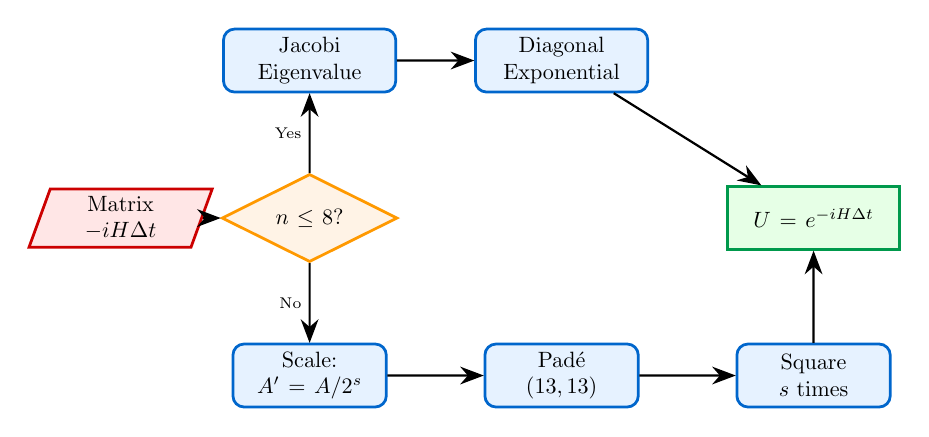
\begin{tikzpicture}[node distance=1cm, scale=0.8, transform shape]
    % Input
    \node[io, text width=2cm] (input) at (-6, 0) {Matrix\\$-iH\Delta t$};
    
    % Decision: size check
    \node[decision, text width=1.5cm] (size) at (-3, 0) {$n \leq 8$?};
    
    % Eigendecomposition path
    \node[block, text width=2.5cm] (eigen) at (-3, 2.5) {Jacobi\\Eigenvalue};
    \node[block, text width=2.5cm] (diag) at (1, 2.5) {Diagonal\\Exponential};
    
    % Padé path
    \node[block, text width=2.2cm] (scale) at (-3, -2.5) {Scale:\\$A' = A/2^s$};
    \node[block, text width=2.2cm] (pade) at (1, -2.5) {Padé\\$(13,13)$};
    \node[block, text width=2.2cm] (square) at (5, -2.5) {Square\\$s$ times};
    
    % Merge
    \node[process, text width=2.5cm] (output) at (5, 0) {$U = e^{-iH\Delta t}$};
    
    % Arrows
    \draw[arrow] (input) -- (size);
    \draw[arrow] (size) -- (eigen) node[midway, left, font=\scriptsize] {Yes};
    \draw[arrow] (eigen) -- (diag);
    \draw[arrow] (diag) -- (output);
    \draw[arrow] (size) -- (scale) node[midway, left, font=\scriptsize] {No};
    \draw[arrow] (scale) -- (pade);
    \draw[arrow] (pade) -- (square);
    \draw[arrow] (square) -- (output);
\end{tikzpicture}
\caption{Matrix exponential computation strategies based on system size}
\label{fig:matrix-exp}
\end{figure}

\subsubsection{Pulse Waveform Generation}

Realistic pulse shapes require high temporal resolution:

\textbf{Gaussian Pulse:}
\begin{equation}
\Omega_G(t) = A \exp\left(-\frac{(t-t_0)^2}{2\sigma^2}\right)
\label{eq:gaussian}
\end{equation}

\textbf{DRAG (Derivative Removal by Adiabatic Gate) Pulse:}
\begin{equation}
\Omega_{\text{DRAG}}(t) = \Omega_G(t) - i\frac{\beta}{\Delta} \frac{d\Omega_G(t)}{dt}
\label{eq:drag}
\end{equation}

where $\beta$ is the DRAG coefficient and $\Delta$ is the anharmonicity.

\textbf{Hermite-Gaussian Pulse:}
\begin{equation}
\Omega_H(t) = A \cdot H_n\left(\frac{t-t_0}{\sigma}\right) \exp\left(-\frac{(t-t_0)^2}{2\sigma^2}\right)
\label{eq:hermite}
\end{equation}

where $H_n(x)$ is the $n$-th Hermite polynomial.

%% ============ PULSE WAVEFORM EXAMPLES ============
\begin{figure}[htbp]
\centering
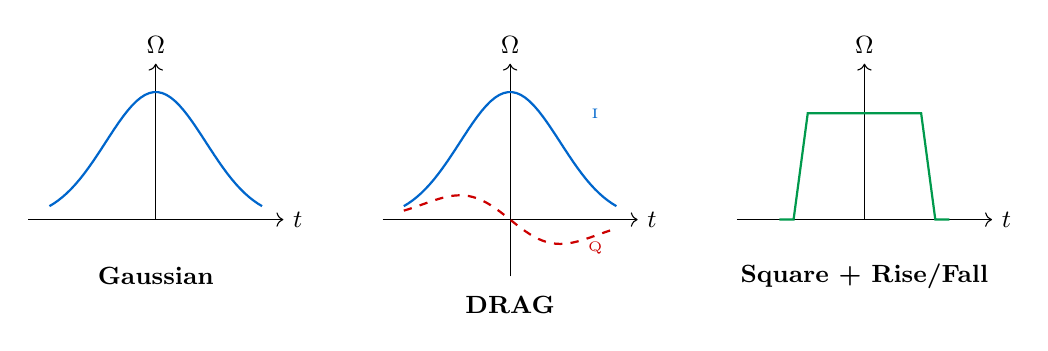
\begin{tikzpicture}[scale=0.9]
    % Gaussian
    \begin{scope}[shift={(-5,0)}]
        \draw[->] (-1.8,0) -- (1.8,0) node[right] {\small $t$};
        \draw[->] (0,0) -- (0,2.2) node[above] {\small $\Omega$};
        \draw[thick, cdacblue, domain=-1.5:1.5, samples=50] plot (\x, {1.8*exp(-\x*\x)});
        \node[font=\small\bfseries] at (0,-0.8) {Gaussian};
    \end{scope}
    
    % DRAG (In-phase and Quadrature)
    \begin{scope}[shift={(0,0)}]
        \draw[->] (-1.8,0) -- (1.8,0) node[right] {\small $t$};
        \draw[->] (0,-0.8) -- (0,2.2) node[above] {\small $\Omega$};
        \draw[thick, cdacblue, domain=-1.5:1.5, samples=50] plot (\x, {1.8*exp(-\x*\x)});
        \draw[thick, nodered, dashed, domain=-1.5:1.5, samples=50] plot (\x, {-0.8*\x*exp(-\x*\x)});
        \node[font=\small\bfseries] at (0,-1.2) {DRAG};
        \node[font=\tiny, cdacblue] at (1.2,1.5) {I};
        \node[font=\tiny, nodered] at (1.2,-0.4) {Q};
    \end{scope}
    
    % Square with rise/fall
    \begin{scope}[shift={(5,0)}]
        \draw[->] (-1.8,0) -- (1.8,0) node[right] {\small $t$};
        \draw[->] (0,0) -- (0,2.2) node[above] {\small $\Omega$};
        \draw[thick, quantumgreen] (-1.2,0) -- (-1,0) -- (-0.8,1.5) -- (0.8,1.5) -- (1,0) -- (1.2,0);
        \node[font=\small\bfseries] at (0,-0.8) {Square + Rise/Fall};
    \end{scope}
\end{tikzpicture}
\caption{Supported pulse waveform shapes: Gaussian, DRAG (with I and Q components), and square with finite rise/fall times}
\label{fig:pulses}
\end{figure}

\subsection{Phase 2 Implementation: Noise and Decoherence (Year 2)}

\subsubsection{Density Matrix Formalism}

For open quantum systems, we transition from pure states $|\psi\rangle$ to density matrices $\rho$:
\begin{equation}
\rho = \sum_i p_i |\psi_i\rangle\langle\psi_i|, \quad \text{Tr}(\rho) = 1, \quad \rho \geq 0
\label{eq:density-matrix}
\end{equation}

The Lindblad master equation governs the evolution:
\begin{equation}
\frac{d\rho}{dt} = -\frac{i}{\hbar}[H(t), \rho] + \sum_k \gamma_k \left(L_k \rho L_k^\dagger - \frac{1}{2}\{L_k^\dagger L_k, \rho\}\right)
\label{eq:lindblad-full}
\end{equation}

%% ============ LINDBLAD SOLVER FLOW DIAGRAM ============
\begin{figure}[htbp]
\centering
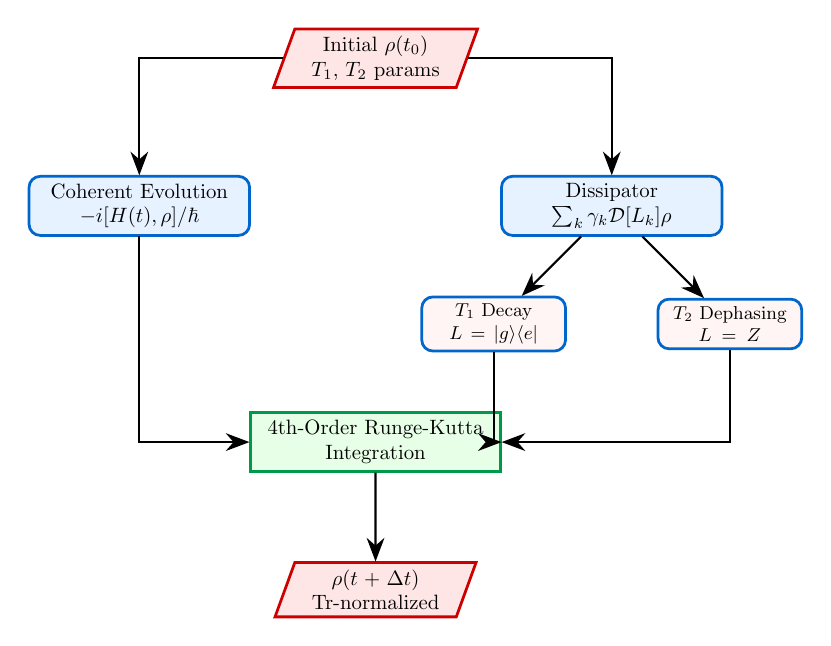
\begin{tikzpicture}[node distance=1cm, scale=0.75, transform shape]
    % Input
    \node[io, text width=2.5cm] (input) at (0, 5) {Initial $\rho(t_0)$\\$T_1$, $T_2$ params};
    
    % Compute coherent part
    \node[block, text width=3.5cm] (coherent) at (-4, 2.5) {Coherent Evolution\\$-i[H(t), \rho]/\hbar$};
    
    % Compute dissipator
    \node[block, text width=3.5cm] (dissip) at (4, 2.5) {Dissipator\\$\sum_k \gamma_k \mathcal{D}[L_k]\rho$};
    
    % Lindblad operators
    \node[smallblock, fill=lightred!40, text width=2.2cm] (t1) at (2, 0.5) {$T_1$ Decay\\$L = |g\rangle\langle e|$};
    \node[smallblock, fill=lightred!40, text width=2.2cm] (t2) at (6, 0.5) {$T_2$ Dephasing\\$L = Z$};
    
    % RK4 Integration
    \node[process, text width=4cm] (rk4) at (0, -1.5) {4th-Order Runge-Kutta\\Integration};
    
    % Output
    \node[io, text width=2.5cm] (output) at (0, -4) {$\rho(t + \Delta t)$\\Tr-normalized};
    
    % Arrows
    \draw[arrow] (input) -| (coherent);
    \draw[arrow] (input) -| (dissip);
    \draw[arrow] (dissip) -- (t1);
    \draw[arrow] (dissip) -- (t2);
    \draw[arrow] (coherent) |- (rk4);
    \draw[arrow] (t1) |- (rk4);
    \draw[arrow] (t2) |- (rk4);
    \draw[arrow] (rk4) -- (output);
\end{tikzpicture}
\caption{Lindblad master equation solver flow diagram with decoherence channels}
\label{fig:lindblad-flow}
\end{figure}

\subsubsection{Decoherence Channel Implementation}

\textbf{Amplitude Damping ($T_1$ process):}
\begin{equation}
L_i^{\text{AD}} = \sqrt{\gamma_1} |g\rangle_i \langle e|_i, \quad \gamma_1 = \frac{1}{T_1}
\label{eq:t1}
\end{equation}

This models energy relaxation from excited state $|e\rangle$ to ground state $|g\rangle$.

\textbf{Pure Dephasing (contributing to $T_2$):}
\begin{equation}
L_i^{\text{PD}} = \sqrt{\gamma_\phi} Z_i, \quad \gamma_\phi = \frac{1}{T_2} - \frac{1}{2T_1}
\label{eq:t2}
\end{equation}

The relationship between $T_1$, $T_2$, and pure dephasing time $T_\phi$ is:
\begin{equation}
\frac{1}{T_2} = \frac{1}{2T_1} + \frac{1}{T_\phi}
\label{eq:t2-relation}
\end{equation}

\subsubsection{Crosstalk Modeling}

Simultaneous pulses on neighboring qubits induce crosstalk:
\begin{equation}
H_{\text{crosstalk}} = \sum_{i \neq j} \xi_{ij} \Omega_i(t) O_j
\label{eq:crosstalk}
\end{equation}

where $\xi_{ij}$ is the crosstalk coefficient matrix (typically 1-5\% for nearest neighbors).

%% ============ CROSSTALK DIAGRAM ============
\begin{figure}[htbp]
\centering
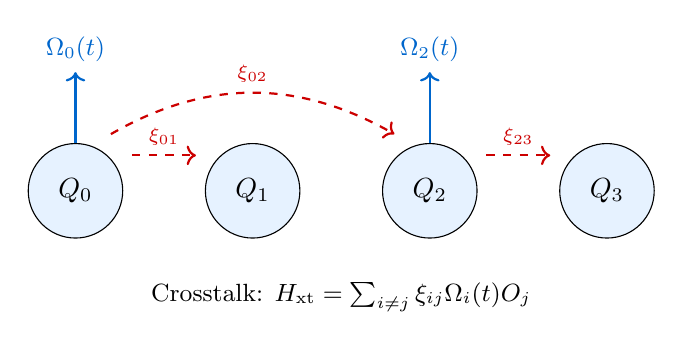
\begin{tikzpicture}[scale=0.9]
    % Qubits
    \foreach \i in {0,1,2,3} {
        \node[draw, circle, minimum size=1.2cm, fill=lightblue] (q\i) at (\i*2.5, 0) {$Q_\i$};
    }
    
    % Intended pulses
    \draw[thick, cdacblue, ->] (q0.north) -- ++(0, 1) node[above, font=\small] {$\Omega_0(t)$};
    \draw[thick, cdacblue, ->] (q2.north) -- ++(0, 1) node[above, font=\small] {$\Omega_2(t)$};
    
    % Crosstalk arrows
    \draw[thick, nodered, ->, dashed] (0.8, 0.5) -- (1.7, 0.5) node[midway, above, font=\scriptsize] {$\xi_{01}$};
    \draw[thick, nodered, ->, dashed] (5.8, 0.5) -- (6.7, 0.5) node[midway, above, font=\scriptsize] {$\xi_{23}$};
    \draw[thick, nodered, ->, dashed, bend left=30] (0.5, 0.8) to node[above, font=\scriptsize] {$\xi_{02}$} (4.5, 0.8);
    
    % Legend
    \node[font=\small] at (3.75, -1.5) {Crosstalk: $H_{\text{xt}} = \sum_{i\neq j} \xi_{ij} \Omega_i(t) O_j$};
\end{tikzpicture}
\caption{Crosstalk between qubits during simultaneous pulse application}
\label{fig:crosstalk}
\end{figure}

\subsection{Phase 3 Implementation: Integration and Optimization (Year 3)}

\subsubsection{Qiskit Pulse Backend Integration}

The simulator implements the Qiskit \texttt{PulseBackend} interface:

%% ============ QISKIT INTEGRATION DIAGRAM ============
\begin{figure}[htbp]
\centering
\begin{tikzpicture}[node distance=1cm, scale=0.8, transform shape]
    % Qiskit side
    \node[wideblock, fill=lightorange!50] (schedule) at (-4, 3) {Qiskit Pulse\\Schedule};
    \node[wideblock, fill=lightorange!50] (backend) at (-4, 1) {Backend\\Configuration};
    \node[wideblock, fill=lightorange!50] (calib) at (-4, -1) {Calibration\\Data};
    
    % Parser
    \node[process, text width=3cm, minimum height=2.5cm] (parser) at (0, 1) {Pulse Schedule\\Parser\\\\Instructions:\\Play, Delay,\\ShiftPhase,\\SetFrequency,\\Acquire};
    
    % FPGA instructions
    \node[block, text width=3.5cm] (fpga) at (4, 1) {FPGA Instruction\\Stream};
    
    % Execution
    \node[process, text width=3cm] (exec) at (8, 1) {FPGA\\Execution};
    
    % Results
    \node[io, text width=2.5cm] (result) at (8, -2) {Qiskit Result\\Object};
    
    % Arrows
    \draw[arrow] (schedule) -- (parser);
    \draw[arrow] (backend) -- (parser);
    \draw[arrow] (calib) -- (parser);
    \draw[arrow] (parser) -- (fpga);
    \draw[arrow] (fpga) -- (exec);
    \draw[arrow] (exec) -- (result);
    
    % Return path
    \draw[dashedarrow] (result) -| (-4, -2.5) -| (schedule);
\end{tikzpicture}
\caption{Qiskit Pulse backend integration architecture}
\label{fig:qiskit-integration}
\end{figure}

\subsubsection{Pulse Optimization: GRAPE Algorithm}

Gradient Ascent Pulse Engineering (GRAPE) optimizes pulse sequences for target unitary operations:

\textbf{Objective Function:}
\begin{equation}
F = \frac{1}{d^2}\left|\text{Tr}\left(U_{\text{target}}^\dagger U_{\text{pulse}}\right)\right|^2
\label{eq:grape-fidelity}
\end{equation}

\textbf{Gradient Computation:}
\begin{equation}
\frac{\partial F}{\partial \Omega_k(t_j)} = \frac{2}{d^2} \text{Re}\left[\text{Tr}\left(U_{\text{target}}^\dagger \frac{\partial U_{\text{pulse}}}{\partial \Omega_k(t_j)}\right) \text{Tr}\left(U_{\text{pulse}}^\dagger U_{\text{target}}\right)^*\right]
\label{eq:grape-gradient}
\end{equation}

The gradient with respect to pulse amplitude at time slice $j$ involves:
\begin{equation}
\frac{\partial U_{\text{pulse}}}{\partial \Omega_k(t_j)} = U(t_N, t_{j+1}) \left(-\frac{i\Delta t}{\hbar} H_k\right) U(t_j, t_0)
\label{eq:grape-unitary-grad}
\end{equation}

%% ============ GRAPE OPTIMIZATION FLOW ============
\begin{figure}[htbp]
\centering
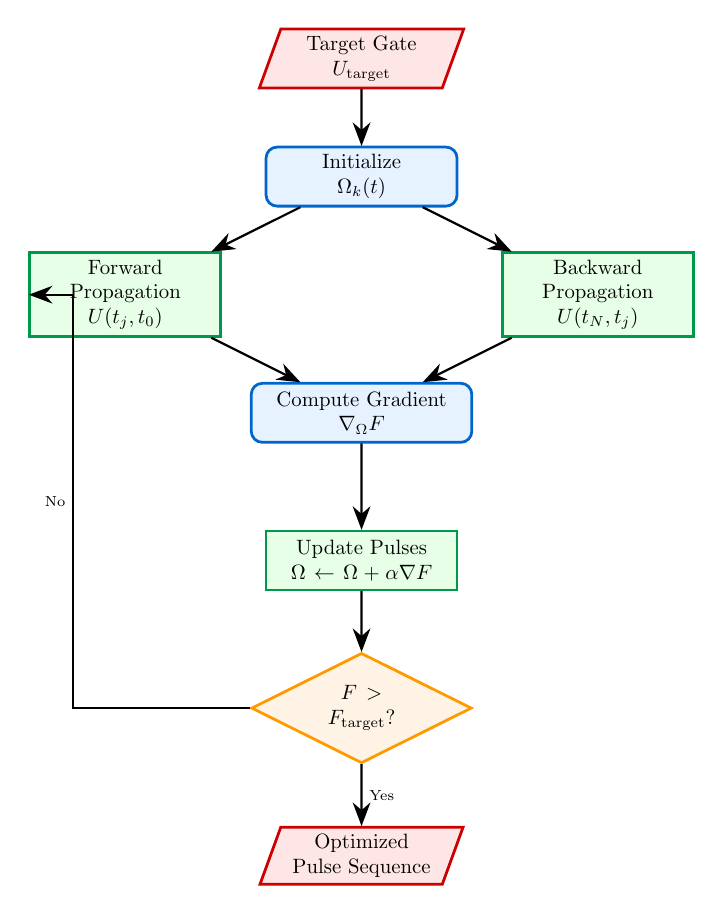
\begin{tikzpicture}[node distance=1cm, scale=0.75, transform shape]
    % Start
    \node[io, text width=2.5cm] (start) at (0, 5) {Target Gate\\$U_{\text{target}}$};
    
    % Initialize pulses
    \node[block] (init) at (0, 3) {Initialize\\$\Omega_k(t)$};
    
    % Forward propagation
    \node[process, text width=3cm] (forward) at (-4, 1) {Forward\\Propagation\\$U(t_j, t_0)$};
    
    % Backward propagation
    \node[process, text width=3cm] (backward) at (4, 1) {Backward\\Propagation\\$U(t_N, t_j)$};
    
    % Compute gradient
    \node[block, text width=3.5cm] (grad) at (0, -1) {Compute Gradient\\$\nabla_\Omega F$};
    
    % Update pulses
    \node[process, text width=3cm] (update) at (0, -3.5) {Update Pulses\\$\Omega \leftarrow \Omega + \alpha\nabla F$};
    
    % Convergence check
    \node[decision, text width=1.5cm] (conv) at (0, -6) {$F > F_{\text{target}}$?};
    
    % Output
    \node[io, text width=2.5cm] (output) at (0, -8.5) {Optimized\\Pulse Sequence};
    
    % Arrows
    \draw[arrow] (start) -- (init);
    \draw[arrow] (init) -- (forward);
    \draw[arrow] (init) -- (backward);
    \draw[arrow] (forward) -- (grad);
    \draw[arrow] (backward) -- (grad);
    \draw[arrow] (grad) -- (update);
    \draw[arrow] (update) -- (conv);
    \draw[arrow] (conv) -- (output) node[midway, right, font=\scriptsize] {Yes};
    \draw[arrow] (conv.west) -- ++(-3,0) |- (forward.west) node[pos=0.25, left, font=\scriptsize] {No};
\end{tikzpicture}
\caption{GRAPE pulse optimization algorithm flow diagram}
\label{fig:grape-flow}
\end{figure}

\newpage
\section{Quarterly Milestones and Timeline}

%% ============ GANTT CHART FOR 3-YEAR TIMELINE ============
\begin{figure}[htbp]
\centering
\resizebox{\textwidth}{!}{
\begin{ganttchart}[
    hgrid,
    vgrid,
    x unit=0.45cm,
    y unit chart=0.6cm,
    y unit title=0.8cm,
    title height=1,
    bar height=0.6,
    bar label font=\scriptsize,
    group label font=\small\bfseries,
    milestone label font=\scriptsize\bfseries,
    title label font=\small\bfseries,
    bar/.append style={fill=cdacblue!60},
    group/.append style={fill=quantumgreen!40},
    milestone/.append style={fill=nodered}
]{1}{12}
    \gantttitle{Year 1: Core Engine}{4}
    \gantttitle{Year 2: Noise \& Decoherence}{4}
    \gantttitle{Year 3: Integration}{4} \\
    \gantttitlelist{Q1,Q2,Q3,Q4,Q5,Q6,Q7,Q8,Q9,Q10,Q11,Q12}{1} \\
    
    % Year 1
    \ganttgroup{Phase 1: Evolution Engine}{1}{4} \\
    \ganttbar{System Design}{1}{1} \\
    \ganttbar{Hamiltonian Engine}{2}{2} \\
    \ganttbar{Waveform Engine}{3}{3} \\
    \ganttbar{Matrix Exponential Opt.}{4}{4} \\
    \ganttmilestone{8-Qubit Demo}{4} \\
    
    % Year 2
    \ganttgroup{Phase 2: Noise Modeling}{5}{8} \\
    \ganttbar{Density Matrix Framework}{5}{5} \\
    \ganttbar{Noise Injection Module}{6}{6} \\
    \ganttbar{Crosstalk Modeling}{7}{7} \\
    \ganttbar{12-Qubit Scaling}{8}{8} \\
    \ganttmilestone{12-Qubit + Noise Demo}{8} \\
    
    % Year 3
    \ganttgroup{Phase 3: Integration}{9}{12} \\
    \ganttbar{Qiskit Backend}{9}{9} \\
    \ganttbar{Qniverse Deployment}{10}{10} \\
    \ganttbar{Pulse Optimization Tools}{11}{11} \\
    \ganttbar{Benchmarking \& Validation}{12}{12} \\
    \ganttmilestone{Production Release}{12}
    
    % Links
    \ganttlink{elem1}{elem2}
    \ganttlink{elem2}{elem3}
    \ganttlink{elem3}{elem4}
    \ganttlink{elem6}{elem7}
    \ganttlink{elem7}{elem8}
    \ganttlink{elem8}{elem9}
    \ganttlink{elem11}{elem12}
    \ganttlink{elem12}{elem13}
    \ganttlink{elem13}{elem14}
\end{ganttchart}
}
\caption{Three-year project timeline with quarterly milestones}
\label{fig:gantt}
\end{figure}

\subsection{Year 1: Core Pulse Evolution Engine}

\textbf{Quarter 1 (Months 1-3): System Design and Architecture}
\begin{itemize}[noitemsep]
    \item Complete system architecture document with FPGA resource allocation
    \item Finalize Hamiltonian representation and storage scheme
    \item Design memory distribution for 32 HBM banks
    \item Procure Xilinx Alveo U55C and establish development environment
    \item \textbf{Deliverable:} System Design Document (150+ pages)
\end{itemize}

\textbf{Quarter 2 (Months 4-6): Hamiltonian Engine}
\begin{itemize}[noitemsep]
    \item Implement Hamiltonian matrix construction in HLS
    \item Develop sparse matrix storage (CRS format)
    \item Create basic 2nd-order Magnus expansion
    \item Validate: 2-qubit Rabi oscillations
    \item \textbf{Milestone:} 2-Qubit simulation functional
\end{itemize}

\textbf{Quarter 3 (Months 7-9): Waveform Engine}
\begin{itemize}[noitemsep]
    \item Implement Gaussian, square, DRAG pulse generators
    \item Develop adaptive time-stepping
    \item Create pulse schedule compiler
    \item Extend to 4-qubit systems
    \item \textbf{Milestone:} 4-Qubit time-dependent simulation
\end{itemize}

\textbf{Quarter 4 (Months 10-12): Optimization and Scaling}
\begin{itemize}[noitemsep]
    \item Implement 4th-order Magnus expansion
    \item Optimize Padé (13,13) matrix exponential
    \item Scale to 8-qubit systems
    \item Benchmark against QuTiP
    \item \textbf{Milestone:} 8-Qubit pulse circuit execution
\end{itemize}

\subsection{Year 2: Noise Modeling and Decoherence}

\textbf{Quarter 5 (Months 13-15): Density Matrix Framework}
\begin{itemize}[noitemsep]
    \item Transition to density matrix representation
    \item Implement Lindblad master equation solver
    \item Add $T_1$, $T_2$ decoherence operators
    \item Extend to 6-qubit open systems
    \item \textbf{Milestone:} 6-Qubit open system dynamics
\end{itemize}

\textbf{Quarter 6 (Months 16-18): Control Noise}
\begin{itemize}[noitemsep]
    \item Implement on-FPGA PRNG (Xoroshiro128+)
    \item Develop amplitude, phase, timing noise modules
    \item Create $1/f$ noise generator
    \item Validate noise statistics
    \item \textbf{Milestone:} Realistic control noise operational
\end{itemize}

\textbf{Quarter 7 (Months 19-21): Crosstalk}
\begin{itemize}[noitemsep]
    \item Implement crosstalk matrix framework
    \item Model capacitive/inductive crosstalk
    \item Validate against IBM/Google hardware data
    \item Extend to 10-qubit with crosstalk
    \item \textbf{Milestone:} 10-Qubit with crosstalk and noise
\end{itemize}

\textbf{Quarter 8 (Months 22-24): Full Capability}
\begin{itemize}[noitemsep]
    \item Scale to 12 qubits (256 MB density matrix)
    \item Optimize HBM access patterns
    \item Complete noise characterization suite
    \item End-to-end benchmarking
    \item \textbf{Milestone:} 12-Qubit pulse simulation with realistic noise
\end{itemize}

\subsection{Year 3: Integration and Deployment}

\textbf{Quarter 9 (Months 25-27): Qiskit Integration}
\begin{itemize}[noitemsep]
    \item Implement Qiskit \texttt{PulseBackend} interface
    \item Develop pulse schedule parser
    \item Support all Qiskit Pulse instructions
    \item \textbf{Milestone:} Seamless Qiskit Pulse integration
\end{itemize}

\textbf{Quarter 10 (Months 28-30): Qniverse Deployment}
\begin{itemize}[noitemsep]
    \item Integrate as Qniverse Platform backend
    \item Develop web-based pulse composer UI
    \item Implement job queue management
    \item Beta testing with 50+ users
    \item \textbf{Milestone:} Public beta on Qniverse
\end{itemize}

\textbf{Quarter 11 (Months 31-33): Optimization Tools}
\begin{itemize}[noitemsep]
    \item Implement DRAG optimization
    \item Develop GRAPE framework
    \item Create calibration protocols (Rabi, Ramsey, RB)
    \item Build pre-optimized pulse library
    \item \textbf{Milestone:} Automated pulse calibration operational
\end{itemize}

\textbf{Quarter 12 (Months 34-36): Validation and Release}
\begin{itemize}[noitemsep]
    \item Comprehensive benchmarking vs. CPU/GPU
    \item Validate against experimental data
    \item Hardware-in-the-loop testing with AWGs
    \item Final documentation and training workshops
    \item \textbf{Milestone:} Production deployment complete
\end{itemize}

\subsection{Timeline Feasibility Analysis}

%% ============ FEASIBILITY ANALYSIS DIAGRAM ============
\begin{figure}[htbp]
\centering
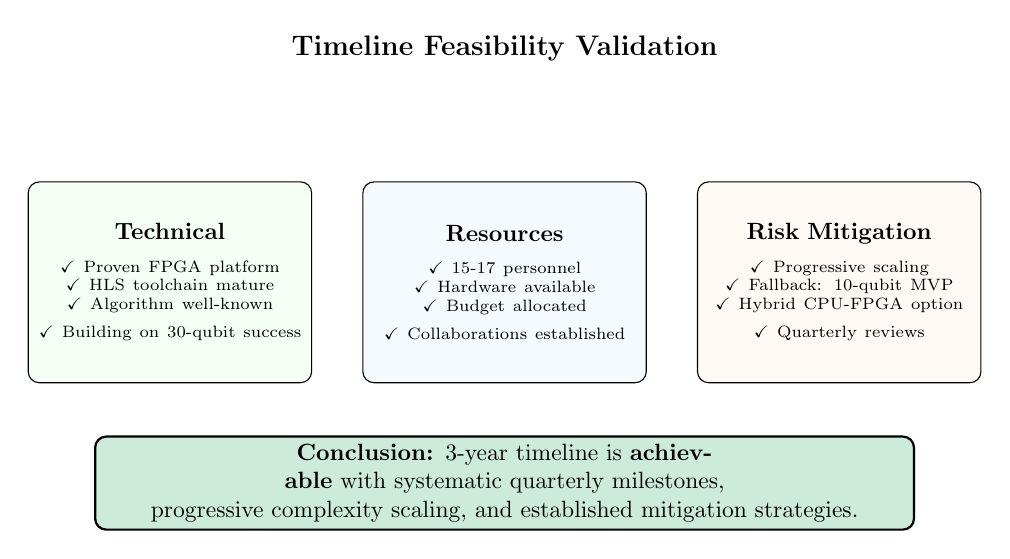
\begin{tikzpicture}[scale=0.85, transform shape]
    % Title
    \node[font=\large\bfseries] at (0, 4.5) {Timeline Feasibility Validation};
    
    % Three pillars
    \node[draw, rounded corners, fill=lightgreen!40, text width=4cm, minimum height=3cm, align=center] (tech) at (-5, 1) {
        \textbf{Technical}\\[0.2cm]
        \scriptsize
        $\checkmark$ Proven FPGA platform\\
        $\checkmark$ HLS toolchain mature\\
        $\checkmark$ Algorithm well-known\\
        $\checkmark$ Building on 30-qubit success
    };
    
    \node[draw, rounded corners, fill=lightblue!40, text width=4cm, minimum height=3cm, align=center] (resource) at (0, 1) {
        \textbf{Resources}\\[0.2cm]
        \scriptsize
        $\checkmark$ 15-17 personnel\\
        $\checkmark$ Hardware available\\
        $\checkmark$ Budget allocated\\
        $\checkmark$ Collaborations established
    };
    
    \node[draw, rounded corners, fill=lightorange!40, text width=4cm, minimum height=3cm, align=center] (risk) at (5, 1) {
        \textbf{Risk Mitigation}\\[0.2cm]
        \scriptsize
        $\checkmark$ Progressive scaling\\
        $\checkmark$ Fallback: 10-qubit MVP\\
        $\checkmark$ Hybrid CPU-FPGA option\\
        $\checkmark$ Quarterly reviews
    };
    
    % Conclusion
    \node[draw, thick, rounded corners, fill=quantumgreen!20, text width=12cm, align=center] at (0, -2) {
        \textbf{Conclusion:} 3-year timeline is \textbf{achievable} with systematic quarterly milestones,\\
        progressive complexity scaling, and established mitigation strategies.
    };
\end{tikzpicture}
\caption{Timeline feasibility analysis based on technical, resource, and risk factors}
\label{fig:feasibility}
\end{figure}

The 3-year timeline is validated based on:

\begin{enumerate}[noitemsep]
    \item \textbf{Prior Success:} C-DAC's 30-qubit gate simulator was completed in similar timeframe
    \item \textbf{Progressive Scaling:} 2 $\rightarrow$ 4 $\rightarrow$ 8 $\rightarrow$ 10 $\rightarrow$ 12 qubits allows early validation
    \item \textbf{Mature Tools:} Vitis HLS, Vivado, and XRT are production-ready
    \item \textbf{Known Algorithms:} Magnus expansion, Padé approximation are well-established
    \item \textbf{Fallback Position:} 10-qubit with full noise modeling is minimum viable product
\end{enumerate}

\newpage
\section{Expected Outcomes and Impact}

\subsection{Technical Outcomes}

\textbf{1. Indigenous Pulse-Level Quantum Simulation Capability}
\begin{itemize}[noitemsep]
    \item First Indian-developed FPGA-based pulse simulator
    \item 12-qubit capacity with sub-nanosecond time resolution
    \item Comprehensive noise modeling matching physical hardware
    \item Production-ready Qiskit and Qniverse integration
\end{itemize}

\textbf{2. Performance Targets}
\begin{itemize}[noitemsep]
    \item 10-100$\times$ speedup over CPU-based simulators for 10-12 qubit systems
    \item Energy efficiency: $<50$ watts for full 12-qubit simulation
    \item Real-time simulation for $\leq 8$ qubit systems
\end{itemize}

\textbf{3. Ecosystem Enablement}
\begin{itemize}[noitemsep]
    \item 500+ Qniverse users with pulse-level access
    \item Cost savings: $>$\$100K annually per research lab
    \item Accelerate quantum algorithm development 5-12$\times$
\end{itemize}

\subsection{Strategic Impact}

%% ============ IMPACT DIAGRAM ============
\begin{figure}[htbp]
\centering
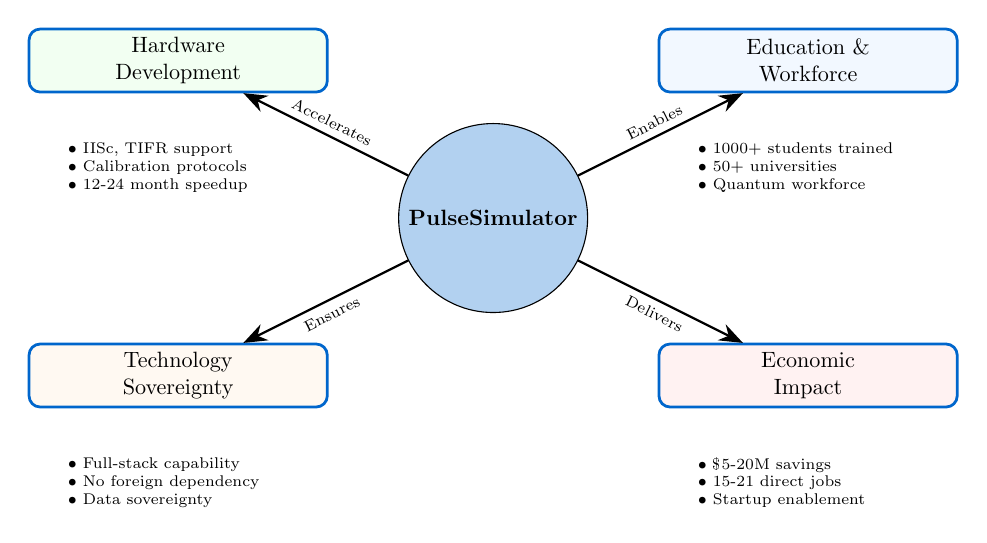
\begin{tikzpicture}[scale=0.8, transform shape]
    % Central node
    \node[draw, circle, fill=cdacblue!30, minimum size=3cm, font=\bfseries] (center) at (0,0) {Pulse\\Simulator};
    
    % Impact areas
    \node[wideblock, fill=lightgreen!50] (hw) at (-5, 2.5) {Hardware\\Development};
    \node[wideblock, fill=lightblue!50] (ed) at (5, 2.5) {Education \&\\Workforce};
    \node[wideblock, fill=lightorange!50] (sov) at (-5, -2.5) {Technology\\Sovereignty};
    \node[wideblock, fill=lightred!50] (eco) at (5, -2.5) {Economic\\Impact};
    
    % Arrows with labels
    \draw[arrow, thick] (center) -- (hw) node[midway, above, sloped, font=\scriptsize] {Accelerates};
    \draw[arrow, thick] (center) -- (ed) node[midway, above, sloped, font=\scriptsize] {Enables};
    \draw[arrow, thick] (center) -- (sov) node[midway, below, sloped, font=\scriptsize] {Ensures};
    \draw[arrow, thick] (center) -- (eco) node[midway, below, sloped, font=\scriptsize] {Delivers};
    
    % Sub-items
    \node[font=\scriptsize, text width=3.5cm, align=left] at (-5, 0.8) {
        $\bullet$ IISc, TIFR support\\
        $\bullet$ Calibration protocols\\
        $\bullet$ 12-24 month speedup
    };
    
    \node[font=\scriptsize, text width=3.5cm, align=left] at (5, 0.8) {
        $\bullet$ 1000+ students trained\\
        $\bullet$ 50+ universities\\
        $\bullet$ Quantum workforce
    };
    
    \node[font=\scriptsize, text width=3.5cm, align=left] at (-5, -4.2) {
        $\bullet$ Full-stack capability\\
        $\bullet$ No foreign dependency\\
        $\bullet$ Data sovereignty
    };
    
    \node[font=\scriptsize, text width=3.5cm, align=left] at (5, -4.2) {
        $\bullet$ \$5-20M savings\\
        $\bullet$ 15-21 direct jobs\\
        $\bullet$ Startup enablement
    };
\end{tikzpicture}
\caption{Strategic impact of the pulse simulator across key national priorities}
\label{fig:impact}
\end{figure}

\newpage
\section{Infrastructure Requirements}

\subsection{Hardware}

\textbf{Development Platform:}
\begin{itemize}[noitemsep]
    \item 2$\times$ Xilinx Alveo U55C FPGA accelerator cards
    \item Host workstations: 2$\times$ servers with PCIe Gen4, 256 GB RAM, 24-core CPUs
\end{itemize}

\textbf{Testing and Validation:}
\begin{itemize}[noitemsep]
    \item 1$\times$ Additional Alveo U55C for independent validation
    \item High-performance CPU cluster (32-core, 512 GB RAM)
    \item GPU server (NVIDIA A100) for comparative benchmarking
\end{itemize}

\textbf{Hardware-in-the-Loop:}
\begin{itemize}[noitemsep]
    \item 1$\times$ Arbitrary Waveform Generator (AWG), $\geq 2$ GSa/s, 10 GHz bandwidth
    \item 1$\times$ High-speed oscilloscope for waveform validation
\end{itemize}

\textbf{Production Deployment:}
\begin{itemize}[noitemsep]
    \item 2$\times$ Production Alveo U55C for Qniverse
    \item Server infrastructure for multi-user job management
\end{itemize}

\subsection{Software Licenses}
\begin{itemize}[noitemsep]
    \item Xilinx Vitis Unified Software Platform
    \item Vivado Design Suite
    \item MATLAB, Mathematica (algorithm prototyping)
    \item ModelSim, Questa (FPGA simulation)
\end{itemize}

\subsection{External Collaborations}
\begin{itemize}[noitemsep]
    \item \textbf{IISc Bangalore:} Superconducting qubit hardware data validation
    \item \textbf{TIFR Mumbai:} Ion trap calibration protocols
    \item \textbf{IIT Madras/Delhi/Bombay:} Algorithm testing
    \item \textbf{QNu Labs, QpiAI:} Application testing and feedback
\end{itemize}

\newpage
\section{Risk Analysis and Mitigation}

%% ============ RISK MATRIX DIAGRAM ============
\begin{figure}[htbp]
\centering
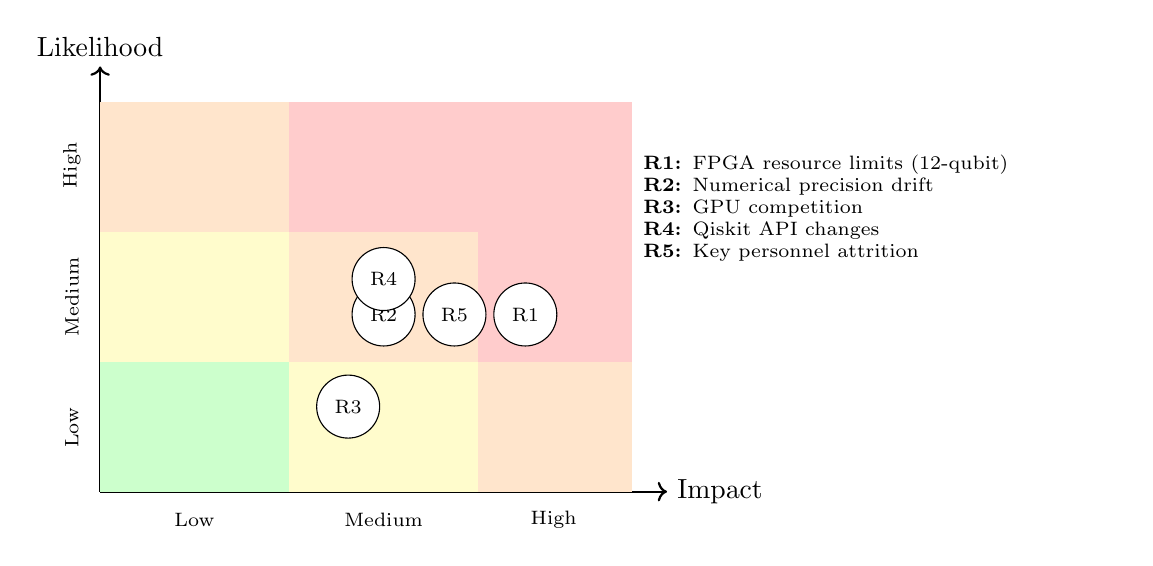
\begin{tikzpicture}[scale=0.9]
    % Axes
    \draw[thick, ->] (0,0) -- (8,0) node[right] {Impact};
    \draw[thick, ->] (0,0) -- (0,6) node[above] {Likelihood};
    
    % Grid
    \draw[gray, dashed] (2.67,0) -- (2.67,5.5);
    \draw[gray, dashed] (5.33,0) -- (5.33,5.5);
    \draw[gray, dashed] (0,1.83) -- (7.5,1.83);
    \draw[gray, dashed] (0,3.67) -- (7.5,3.67);
    
    % Labels
    \node[font=\scriptsize] at (1.33, -0.4) {Low};
    \node[font=\scriptsize] at (4, -0.4) {Medium};
    \node[font=\scriptsize] at (6.4, -0.4) {High};
    \node[font=\scriptsize, rotate=90] at (-0.4, 0.9) {Low};
    \node[font=\scriptsize, rotate=90] at (-0.4, 2.75) {Medium};
    \node[font=\scriptsize, rotate=90] at (-0.4, 4.6) {High};
    
    % Risk zones
    \fill[green!20] (0,0) rectangle (2.67, 1.83);
    \fill[yellow!20] (2.67,0) rectangle (5.33, 1.83);
    \fill[yellow!20] (0,1.83) rectangle (2.67, 3.67);
    \fill[orange!20] (5.33,0) rectangle (7.5, 1.83);
    \fill[orange!20] (2.67,1.83) rectangle (5.33, 3.67);
    \fill[orange!20] (0,3.67) rectangle (2.67, 5.5);
    \fill[red!20] (5.33,1.83) rectangle (7.5, 5.5);
    \fill[red!20] (2.67,3.67) rectangle (5.33, 5.5);
    
    % Risks
    \node[draw, circle, fill=white, minimum size=0.8cm, font=\scriptsize] (r1) at (6, 2.5) {R1};
    \node[draw, circle, fill=white, minimum size=0.8cm, font=\scriptsize] (r2) at (4, 2.5) {R2};
    \node[draw, circle, fill=white, minimum size=0.8cm, font=\scriptsize] (r3) at (3.5, 1.2) {R3};
    \node[draw, circle, fill=white, minimum size=0.8cm, font=\scriptsize] (r4) at (4, 3) {R4};
    \node[draw, circle, fill=white, minimum size=0.8cm, font=\scriptsize] (r5) at (5, 2.5) {R5};
    
    % Legend
    \node[font=\scriptsize, text width=6cm, align=left] at (11, 4) {
        \textbf{R1:} FPGA resource limits (12-qubit)\\
        \textbf{R2:} Numerical precision drift\\
        \textbf{R3:} GPU competition\\
        \textbf{R4:} Qiskit API changes\\
        \textbf{R5:} Key personnel attrition
    };
\end{tikzpicture}
\caption{Risk assessment matrix for project risks}
\label{fig:risk-matrix}
\end{figure}

\subsection{Technical Risks}

\textbf{Risk 1: FPGA Resource Limitations for 12-Qubit}

\textit{Description:} 12-qubit density matrix requires 256 MB; computation may exceed FPGA logic.

\textit{Mitigation:}
\begin{itemize}[noitemsep]
    \item Progressive validation: 8 $\rightarrow$ 10 $\rightarrow$ 12 qubits
    \item Sparse representations where applicable
    \item Hybrid CPU-FPGA offloading
    \item Fallback: 10-qubit as minimum viable product
\end{itemize}

\textbf{Risk 2: Numerical Precision Issues}

\textit{Description:} FP32 may accumulate errors over $>$10,000 time steps.

\textit{Mitigation:}
\begin{itemize}[noitemsep]
    \item Implement FP64 mode for critical simulations
    \item Periodic state renormalization
    \item Comprehensive validation against analytical solutions
\end{itemize}

\textbf{Risk 3: Performance vs. GPU Simulators}

\textit{Description:} Modern GPUs (A100, H100) may outperform FPGA.

\textit{Mitigation:}
\begin{itemize}[noitemsep]
    \item Emphasize energy efficiency and deterministic latency (FPGA advantages)
    \item Target hardware-in-the-loop niche
    \item Highlight deployment flexibility
\end{itemize}

\textbf{Risk 4: Qiskit API Changes}

\textit{Description:} Breaking changes during project timeline.

\textit{Mitigation:}
\begin{itemize}[noitemsep]
    \item Track Qiskit development closely
    \item Maintain abstraction layer
    \item Support multiple Qiskit versions
\end{itemize}

\subsection{Programmatic Risks}

\textbf{Risk 5: Key Personnel Attrition}

\textit{Mitigation:}
\begin{itemize}[noitemsep]
    \item Competitive compensation
    \item Co-authorship opportunities
    \item Comprehensive documentation
    \item Knowledge transfer overlap periods
\end{itemize}

\newpage
\section{Success Metrics}

\subsection{Technical Performance Metrics}

\begin{table}[htbp]
\centering
\begin{tabular}{lcc}
\toprule
\textbf{Metric} & \textbf{Target} & \textbf{Threshold} \\
\midrule
Qubit Capacity & 12 qubits & 10 qubits \\
Time Resolution & 0.5 ns & 1 ns \\
Simulation Speed & $<1$ s per $\mu$s (12 qubits) & $<5$ s per $\mu$s \\
Fidelity Accuracy & $>99.9\%$ vs. analytical & $>99.5\%$ \\
Speedup vs. CPU & 10$\times$ & 3$\times$ \\
Power Consumption & $<50$ W & $<100$ W \\
\bottomrule
\end{tabular}
\caption{Quantitative success metrics with targets and thresholds}
\label{tab:metrics}
\end{table}

\subsection{Ecosystem Impact Metrics}

\begin{itemize}[noitemsep]
    \item \textbf{User Adoption:} 200+ active users within 6 months of deployment
    \item \textbf{Research Enablement:} 10+ publications citing the simulator
    \item \textbf{Educational Impact:} 1,000+ students trained, 10+ universities
    \item \textbf{Industry Engagement:} 3+ Indian quantum startups using simulator
\end{itemize}

\newpage
\section{Alignment with National Quantum Mission}

%% ============ NQM ALIGNMENT DIAGRAM ============
\begin{figure}[htbp]
\centering
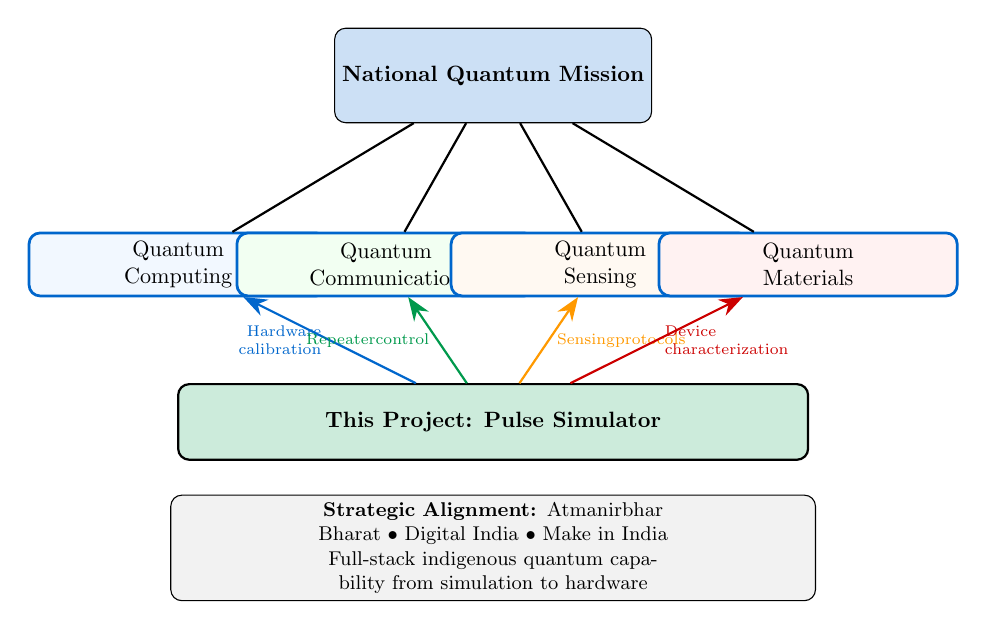
\begin{tikzpicture}[scale=0.8, transform shape]
    % NQM Central
    \node[draw, rounded corners, fill=cdacblue!20, minimum width=4cm, minimum height=1.5cm, font=\bfseries] (nqm) at (0, 4) {National Quantum Mission};
    
    % Pillars
    \node[wideblock, fill=lightblue!50] (qc) at (-5, 1) {Quantum\\Computing};
    \node[wideblock, fill=lightgreen!50] (qcomm) at (-1.7, 1) {Quantum\\Communication};
    \node[wideblock, fill=lightorange!50] (qsens) at (1.7, 1) {Quantum\\Sensing};
    \node[wideblock, fill=lightred!50] (qmat) at (5, 1) {Quantum\\Materials};
    
    % Connections
    \draw[thick] (nqm) -- (qc);
    \draw[thick] (nqm) -- (qcomm);
    \draw[thick] (nqm) -- (qsens);
    \draw[thick] (nqm) -- (qmat);
    
    % Project contribution
    \node[draw, thick, rounded corners, fill=quantumgreen!20, minimum width=10cm, minimum height=1.2cm] (project) at (0, -1.5) {\textbf{This Project: Pulse Simulator}};
    
    % Contribution arrows
    \draw[arrow, thick, cdacblue] (project) -- (qc) node[midway, left, font=\scriptsize, text width=2cm, align=right] {Hardware\\calibration};
    \draw[arrow, thick, quantumgreen] (project) -- (qcomm) node[midway, left, font=\scriptsize] {Repeater\\control};
    \draw[arrow, thick, fpgaorange] (project) -- (qsens) node[midway, right, font=\scriptsize] {Sensing\\protocols};
    \draw[arrow, thick, nodered] (project) -- (qmat) node[midway, right, font=\scriptsize, text width=2cm] {Device\\characterization};
    
    % Additional alignment
    \node[draw, rounded corners, fill=gray!10, text width=10cm, align=center, font=\small] at (0, -3.5) {
        \textbf{Strategic Alignment:} Atmanirbhar Bharat $\bullet$ Digital India $\bullet$ Make in India\\
        Full-stack indigenous quantum capability from simulation to hardware
    };
\end{tikzpicture}
\caption{Project alignment with National Quantum Mission pillars}
\label{fig:nqm-alignment}
\end{figure}

\subsection{Direct Contributions}

\textbf{Quantum Computing Pillar:}
\begin{itemize}[noitemsep]
    \item Accelerates development of 50-100 qubit processors (NQM target)
    \item Provides calibration and optimization infrastructure
    \item Reduces hardware development timeline by 12-24 months
\end{itemize}

\textbf{Technology Sovereignty:}
\begin{itemize}[noitemsep]
    \item Eliminates dependence on IBM, Google, AWS pulse simulation tools
    \item Retains sensitive calibration data within Indian infrastructure
    \item Positions India as quantum technology provider, not consumer
\end{itemize}

\textbf{Workforce Development:}
\begin{itemize}[noitemsep]
    \item Training infrastructure for 1,000+ quantum engineers
    \item Democratizes pulse-level education across Indian institutions
    \item Supports NQM 2030 workforce targets
\end{itemize}

\newpage
\section{Conclusion}

This proposal presents a comprehensive plan for developing an FPGA-based quantum pulse-level simulator that bridges the critical gap between gate-level quantum simulation and physical quantum hardware. Building on C-DAC's proven 30-qubit gate simulator, this project delivers:

\textbf{Technical Innovation:}
\begin{itemize}[noitemsep]
    \item 12-qubit pulse simulation with sub-nanosecond resolution
    \item Comprehensive noise modeling ($T_1$, $T_2$, crosstalk, control noise)
    \item 4th-order Magnus expansion with optimized matrix exponentials
    \item Full Qiskit Pulse and Qniverse integration
\end{itemize}

\textbf{Strategic Value:}
\begin{itemize}[noitemsep]
    \item Completes India's full-stack quantum computing capability
    \item Eliminates foreign tool dependencies
    \item Enables \$5-20M annual savings across Indian quantum ecosystem
    \item Accelerates quantum algorithm development 5-12$\times$
\end{itemize}

\textbf{Feasibility:}
The 3-year timeline is validated through:
\begin{itemize}[noitemsep]
    \item Progressive complexity scaling (2 $\rightarrow$ 12 qubits)
    \item Mature FPGA toolchains and proven platform
    \item Clear quarterly milestones with fallback positions
    \item Established academic and industry collaborations
\end{itemize}

%% ============ SUMMARY VISUAL ============
\begin{figure}[htbp]
\centering
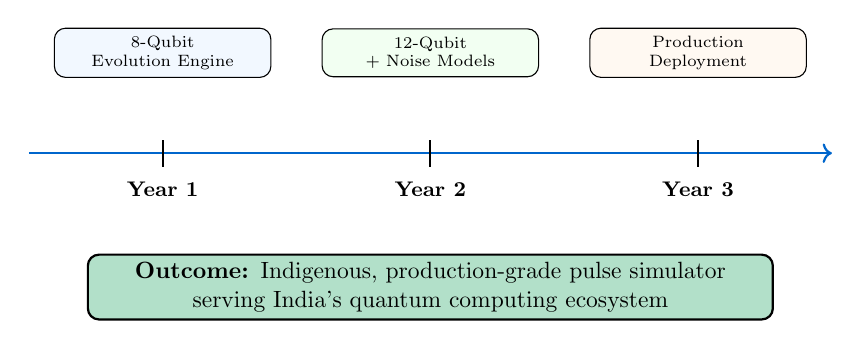
\begin{tikzpicture}[scale=0.85, transform shape]
    % Timeline arrow
    \draw[thick, ->, cdacblue] (-6, 0) -- (6, 0);
    
    % Year markers
    \foreach \x/\label in {-4/Year 1, 0/Year 2, 4/Year 3} {
        \draw[thick] (\x, -0.2) -- (\x, 0.2);
        \node[below, font=\small\bfseries] at (\x, -0.3) {\label};
    }
    
    % Achievements
    \node[draw, rounded corners, fill=lightblue!50, text width=3cm, align=center, font=\scriptsize] at (-4, 1.5) {8-Qubit\\Evolution Engine};
    \node[draw, rounded corners, fill=lightgreen!50, text width=3cm, align=center, font=\scriptsize] at (0, 1.5) {12-Qubit\\+ Noise Models};
    \node[draw, rounded corners, fill=lightorange!50, text width=3cm, align=center, font=\scriptsize] at (4, 1.5) {Production\\Deployment};
    
    % Final outcome
    \node[draw, thick, rounded corners, fill=quantumgreen!30, text width=10cm, align=center] at (0, -2) {
        \textbf{Outcome:} Indigenous, production-grade pulse simulator\\
        serving India's quantum computing ecosystem
    };
\end{tikzpicture}
\caption{Project journey: From concept to production deployment in 3 years}
\label{fig:summary}
\end{figure}

This project delivers production-grade infrastructure for India's quantum computing ecosystem at a critical juncture where pulse-level control distinguishes basic quantum experiments from practical quantum applications. The quantum computing race is not merely about building quantum processors—it is about mastering the entire technology stack from silicon to software. India must control this complete stack to achieve true strategic autonomy in quantum technologies.

\end{document}
